This chapter describes and discusses the results of the running time measurements of the cluster and baseline implementations as described in \ref{chap:implementation}.
\section{ListNet}
Figure \ref{fig:listnet_train_time} and Figure \ref{fig:listnet_train_time_log} (with a logarithmic data size axis) show the processing times of a single training iteration using the ListNet implementation included in RankLib library and the cluster implementation described in chapter \ref{chap:implementation} with different numbers of data nodes.
\begin{figure}
\centering
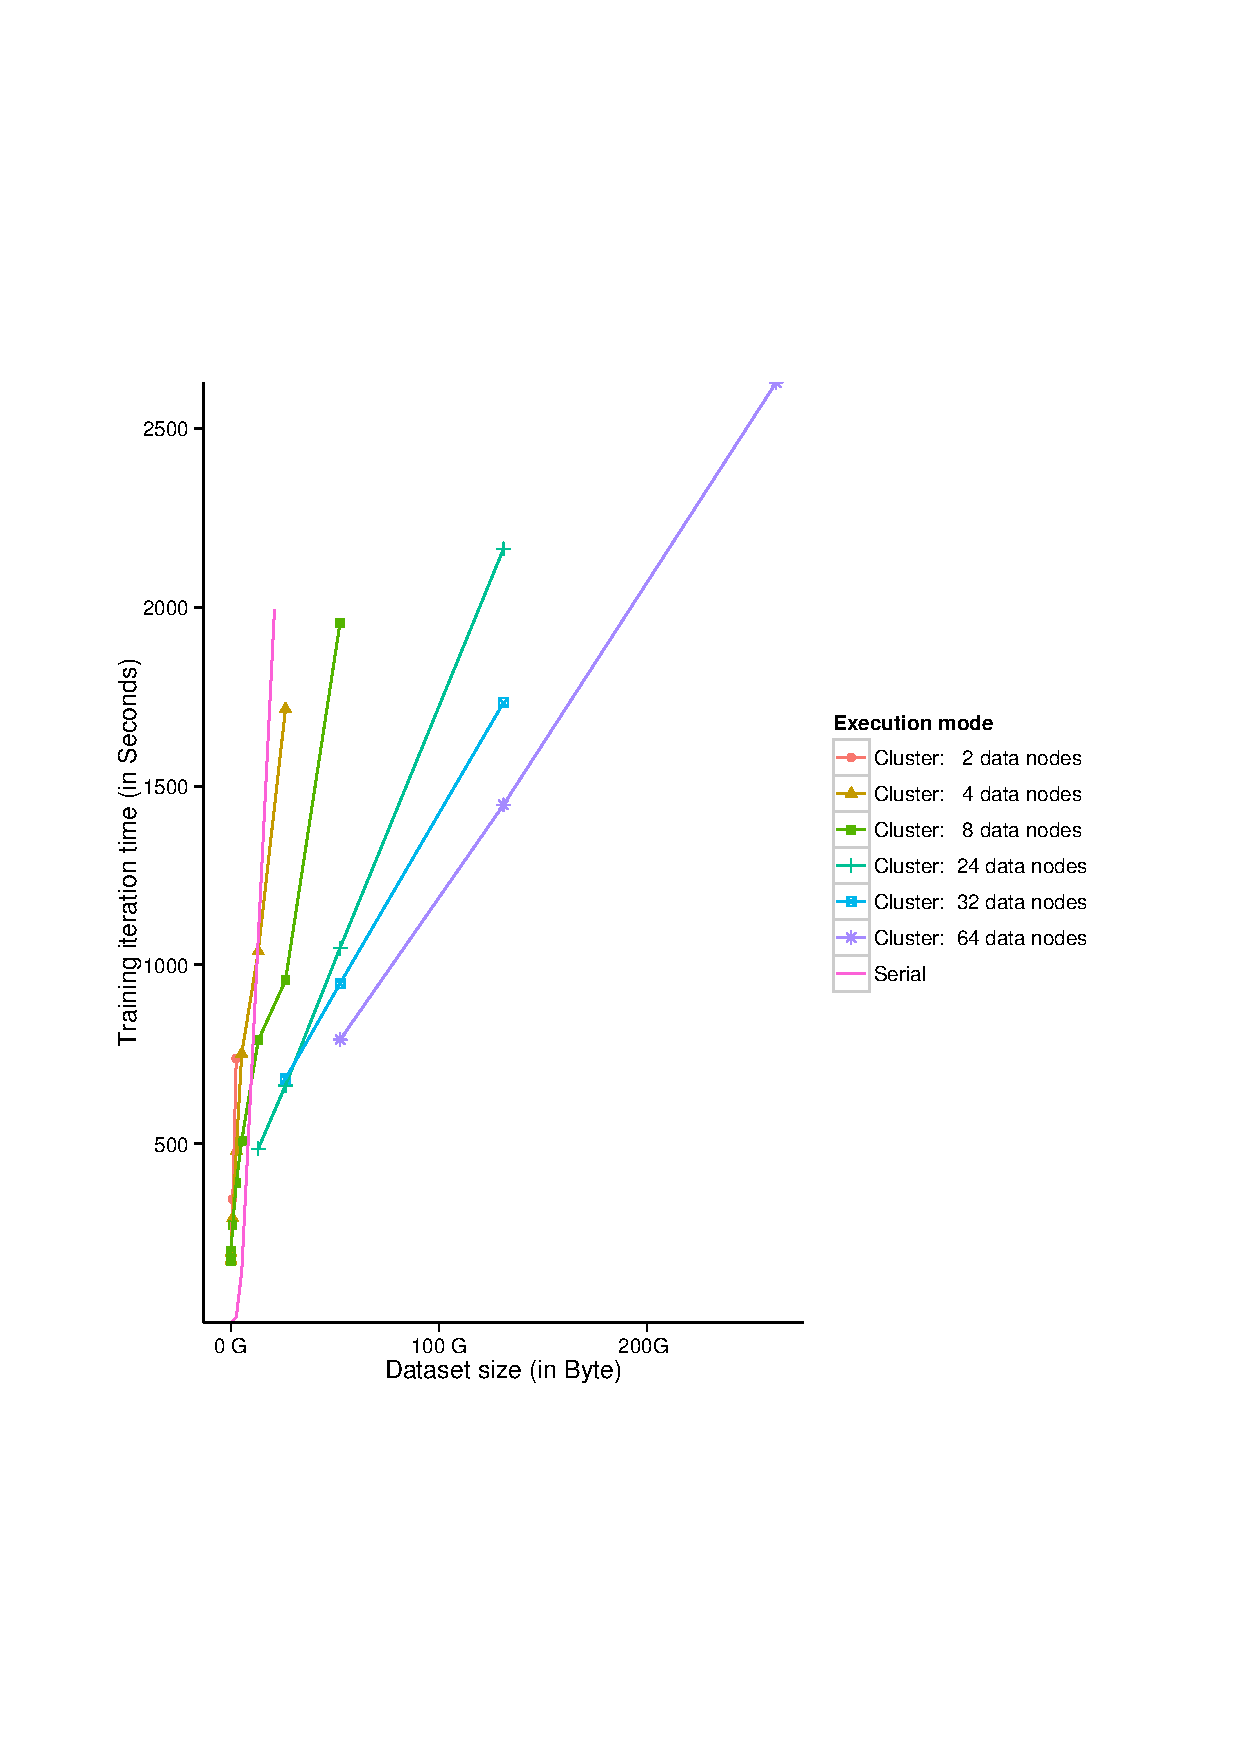
\includegraphics[trim=0cm 5cm 0cm 5cm, scale=0.7]{gfx/time_single.pdf}
\caption{Processing time of a single ListNet training iteration}
\label{fig:listnet_train_time}
\end{figure}

\begin{figure}
\centering
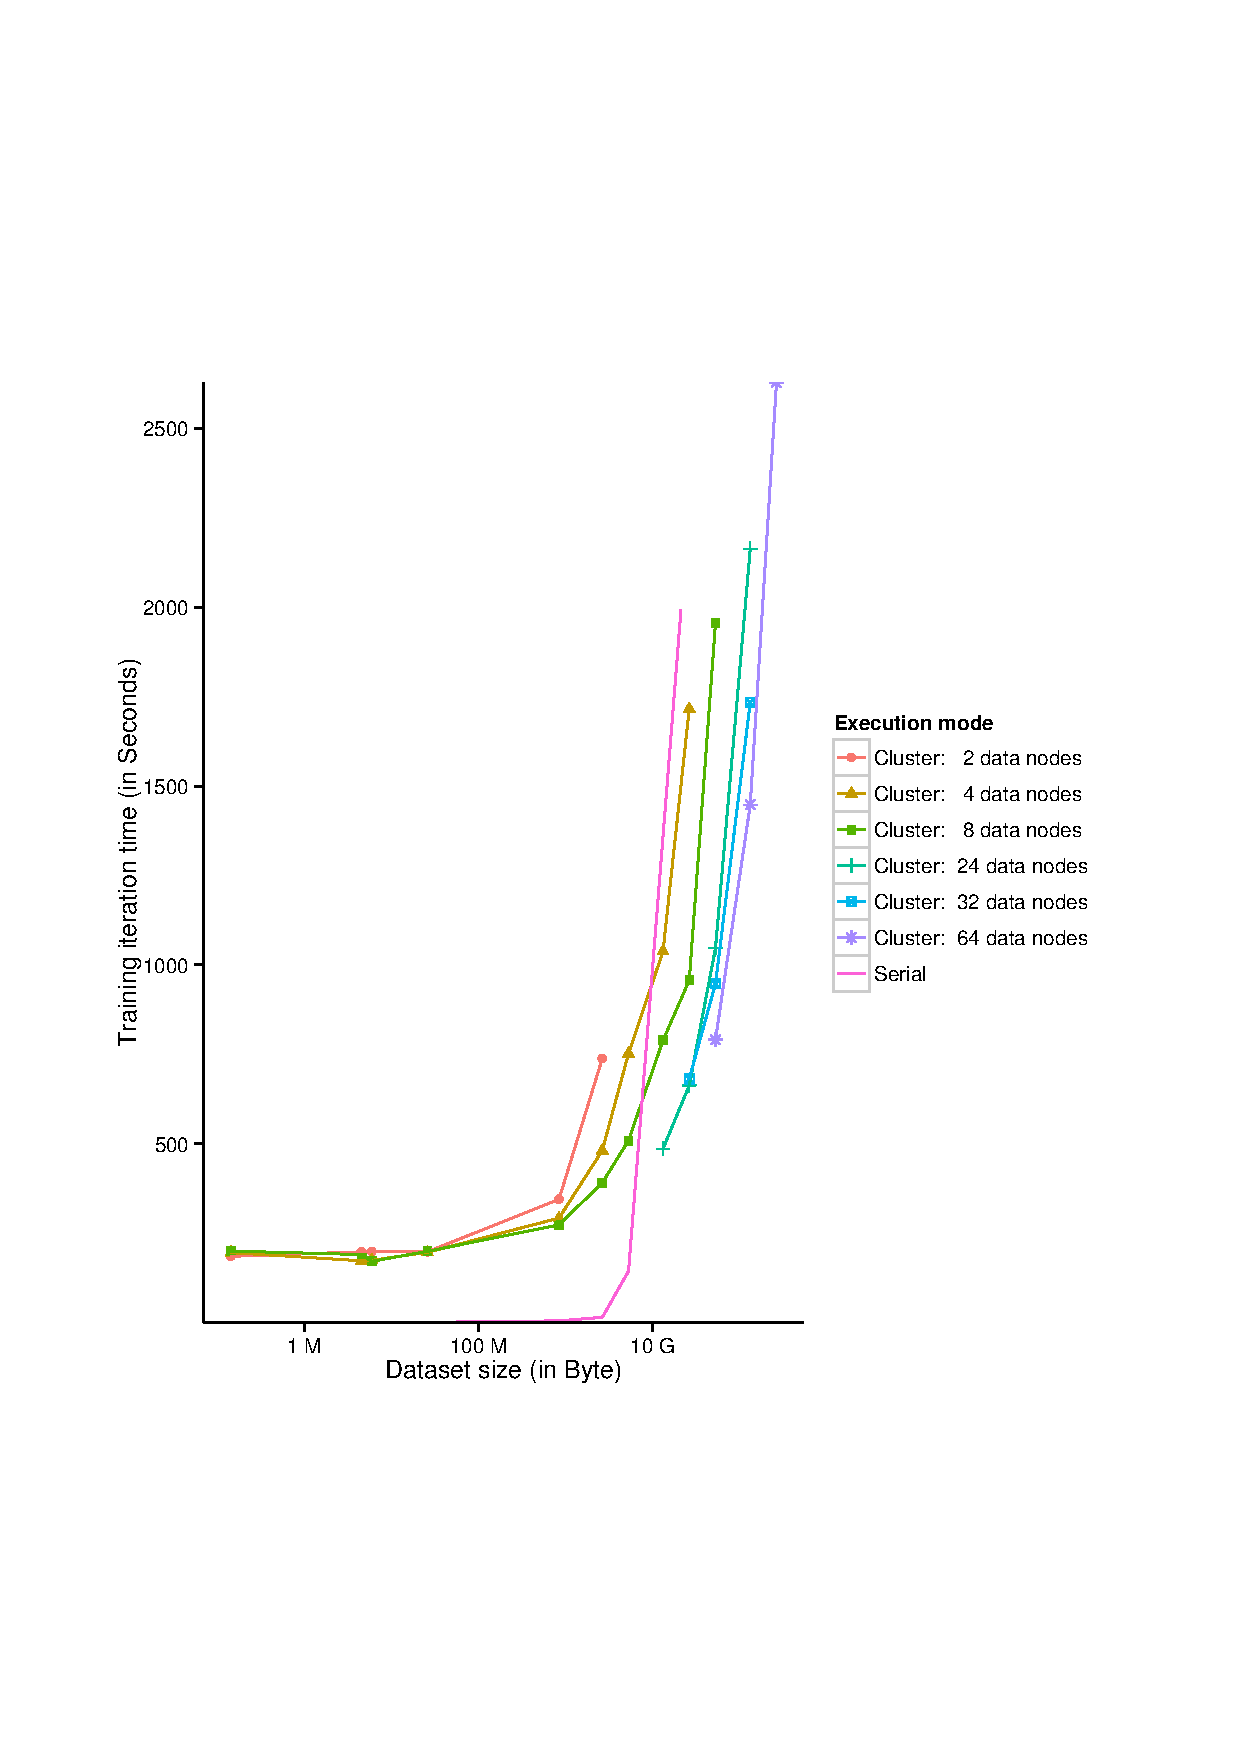
\includegraphics[trim=0cm 5cm 0cm 5cm, scale=0.7]{gfx/time_single_logx.pdf}
\caption{Processing time of a single ListNet training iteration on a logarithmic axis}
\label{fig:listnet_train_time_log}
\end{figure}
Figures \ref{fig:listnet_train_time} and \ref{fig:listnet_train_time_log} also show that serial execution using the RankLib implementation of ListNet is several orders of magnitude faster than running ListNet on a cluster.
\begin{figure}
\centering
\includegraphics[trim=0cm 5cm 0cm 5cm, scale=0.7]{gfx/throughput_single_logx.pdf}
\caption{Throughput of a ListNet training iteration}
\label{fig:listnet_throughput}
\end{figure}